\chapter{Experimental results}
\label{cpt:experiments}

To evaluate Tribler's current situation and to validate our implementations are working correctly, experiments have been conducted.
In this chapter we elaborate on these experiments and discuss the results. 

\section{Performance analysis}
To observe the current situation, we have measured Tribler running idle (i.e. no human interaction) for 4 hours.
For this experiment we run Tribler version 6.6.0-exp1 which is a pre-release of 6.6, because it includes the MultiChain code.
The hardware used during this experiment can be seen in Table \ref{table:tribler_idle}.

\begin{table}[h]
	\centering
	\begin{tabular}{l|l}
		\textbf{Component} 	& \textbf{Specifications} \\ \hline
		Operating System   	& Ubuntu 16.04 LTS \\
		Python version		& 2.7.12 \\
		CPU					& Intel Core i5-2410M \\ 
		HDD					& Samsung 850 EVO 250GB  \\ 
		RAM					& 8 GB DDR3 1600MHz \\
	\end{tabular}
	\caption{Specifications of the setup used during the idle iotop measurement of Tribler 6.6.0-pre-exp.}
	\label{table:tribler_idle}
\end{table}

\begin{figure}[h]
	\makebox[\textwidth][c]{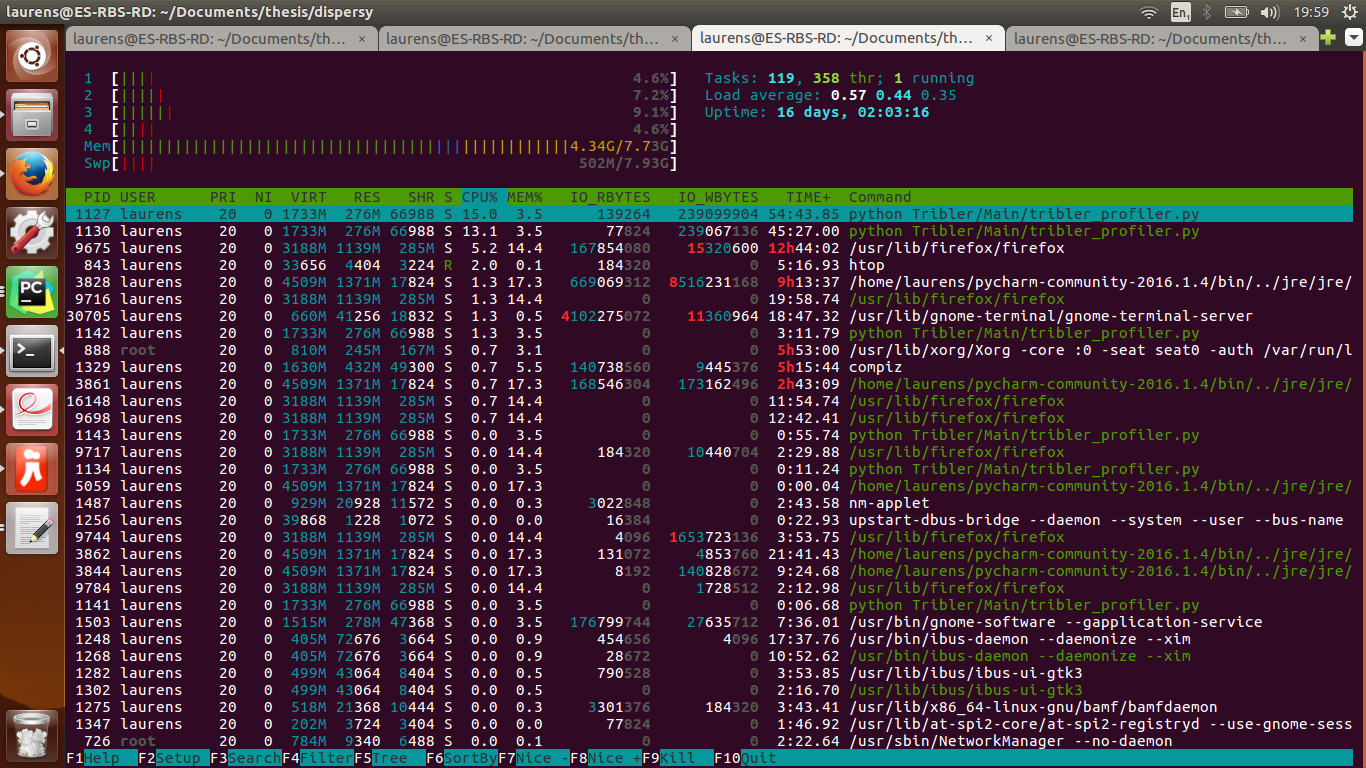
\includegraphics[width=0.95\paperwidth]{experimentation/images/htop.png}}
	\caption{The output of a four hour idle run.}
	\label{fig:htop_io_idle_run}
\end{figure} 

The results are visible in Figure~\ref{fig:htop_io_idle_run}. \todo{cut unity desktop}
From these results we observe that Tribler current has an IO of 144 MB/Hour.

\section{I/O breakdown}

\begin{table}[]
	\centering
	\caption{A breakdown of the functions called on StormDBManager.}
	\label{table:breakdown_tribler_idle}
	\begin{tabular}{|l|r|r|l|l|l|}
		\hline
	\textbf{Query}	& \textbf{Amount of calls} & \textbf{Total time (s)} & \textbf{Max}  & \textbf{Average} & \textbf{Min} \\ \hline
	fetchone	& 83036	& 3361.644 	& 0.81436	& 0.04048	& 0.00006 \\ \hline
	fetchall	& 2569	& 22.512	& 0.66344	& 0.00876	& 0.00007 \\ \hline
	execute		& 422	& 2.326  	& 0.20488	& 0.00551	& 0.00007 \\ \hline
	executemany	& 1		& 0.009 	& 0.00915 	& 0.00915	& 0.00915 \\ \hline
	\end{tabular}
\end{table}

To observe the individual components separately, we have created a breakdown the database queries performed by Tribler and Dispersy.
We have run Tribler idle for one hour on a fresh install and traced how many times each of the five database functions in StormDBManager were being called by either Dispersy or Tribler and how long it takes between scheduling the query and receiving the answer.
A breakdown of these five functions is visible in Table~\ref{table:breakdown_tribler_idle}.
From this table we see that the \enquote{fetchone} function is being called the most, accounting almost for the full duration of the experiment; 56 minutes out of the ~60 minutes.
Previously, this would have been blocking, meaning ~93\% of the time the reactor thread of Tribler would have been blocked.
This demonstrates the urgency of the problem this thesis addresses. 

\section{Validating the performance regression system}

To validate the performance regression system, we have resolved one of Tribler's biggest bottlenecks: Dispersy's blocking database I/O.
To address this problem, we have written Dispersy's I/O to become asynchronous and non-blocking.
To realize this, a new database manager \enquote{StormDBManager} is introduced and 90\%\todo{made up number, need to calculate the actual value.} of Dispersy's functions have been refactored.

